% Requires: \usepackage{booktabs,graphicx,subcaption}
\subsection{Dimension-Matched Gaussian Comparison with SupCon}
\label{subsec:gaussian-supcon}

We compare KDMLP with supervised contrastive learning (SupCon)~\cite{khosla2020supervised}
on a controlled binary Gaussian problem in $d=220$ dimensions.  Let $v\in\mathbb{R}^d$
be a random unit vector and let $A_0,A_1\in\mathbb{R}^{d\times d}$ have independent
standard Gaussian entries.  The class-conditional distributions are
\begin{equation}
 X\mid Y=0\sim\mathcal{N}(-0.1v,\Sigma_0),\qquad
 X\mid Y=1\sim\mathcal{N}(0.1v,\Sigma_1),
 \quad
 \Sigma_0=\frac{A_0^{\top}A_0}{d},\quad
 \Sigma_1=2.5\frac{A_1^{\top}A_1}{d}.
\end{equation}
Thus, $\|\mu_1-\mu_0\|_2=0.2$, whereas
$\|\Sigma_1-\Sigma_0\|_{\mathrm F}=45.538$, so second-order separation is
substantial relative to the mean shift.  In each of two repetitions, we draw
$320$ training, $1200$ test, and $2400$ independent reference observations per
class.

KDMLP and SupCon are evaluated at the same final dimensions $r\in\{1,\ldots,6\}$.
SupCon uses a $128$-dimensional encoder and a $64$-dimensional projection head
inside the contrastive loss; after training, training-set PCA reduces the encoder
output to dimension $r$.  A logistic probe, whose regularization is selected by
three-fold training validation, evaluates both representations.  KDMLP searches
linear, RBF, Laplacian, degree-two polynomial, and sigmoid Stage-1 kernels.

\begin{table}[t]
\centering
\caption{Mean test accuracy over two Gaussian repetitions under the same final
dimension $r$.}
\label{tab:gaussian-supcon-same-r}
\small
\begin{tabular}{c c c c}
\toprule
$r$ & KDMLP-large & KDMLP-small & SupCon \\
\midrule
1 & \textbf{0.9992} & 0.5752 & 0.9471 \\
2 & \textbf{0.9992} & 0.5967 & 0.9479 \\
3 & \textbf{0.9992} & 0.6121 & 0.9475 \\
4 & \textbf{0.9992} & 0.6375 & 0.9469 \\
5 & \textbf{0.9990} & 0.6365 & 0.9483 \\
6 & \textbf{0.9990} & 0.6406 & 0.9492 \\
\bottomrule
\end{tabular}
\end{table}

For method $m$ and dimension $r$, we also report the covariance-gap estimation
error
\begin{equation}
 E_{\Delta C}^{(m,r)}=
 \left\|
 (\widehat C_{1,\mathrm{tr}}^{(m,r)}-\widehat C_{0,\mathrm{tr}}^{(m,r)})-
 (\widehat C_{1,\mathrm{ref}}^{(m,r)}-\widehat C_{0,\mathrm{ref}}^{(m,r)})
 \right\|_{\mathrm F}.
\end{equation}
In the finite-dimensional reduced space, the Frobenius norm equals the
Hilbert--Schmidt norm.  Since each method learns a differently scaled coordinate
system, absolute values of $E_{\Delta C}^{(m,r)}$ are interpreted across $r$
within a method rather than as a direct cross-method ranking.

\begin{figure*}[t]
\centering
\begin{subfigure}{0.49\textwidth}
 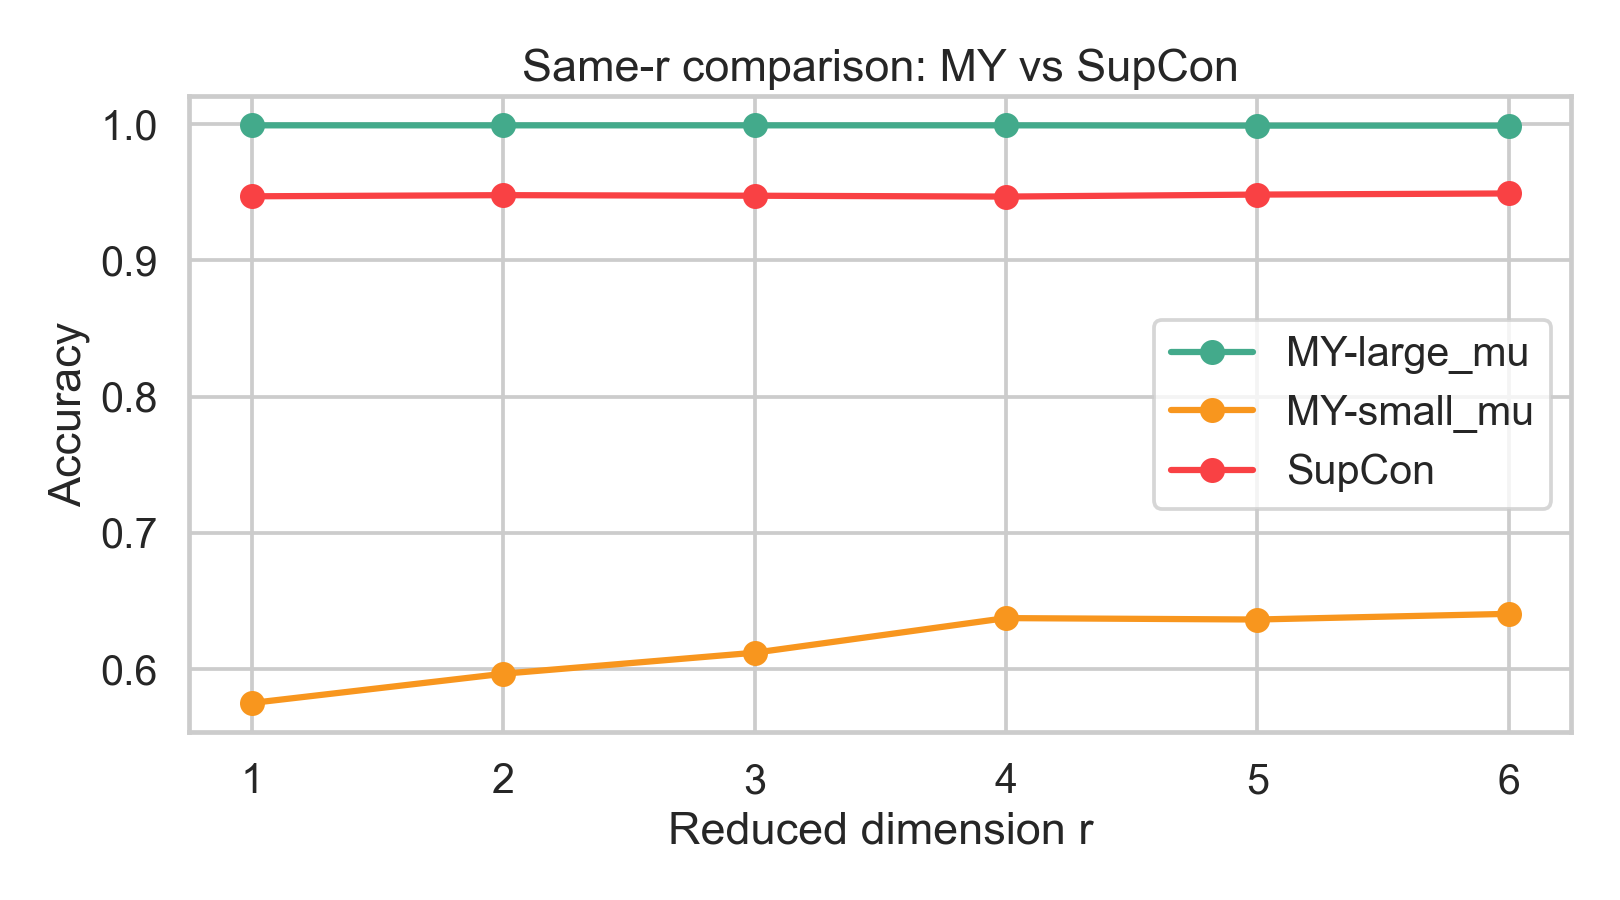
\includegraphics[width=\linewidth]{simulations/supcon_gaussian_workspace/outputs_dimmatch/same_r_accuracy_plot.png}
 \caption{Dimension-matched test accuracy.}
\end{subfigure}
\begin{subfigure}{0.49\textwidth}
 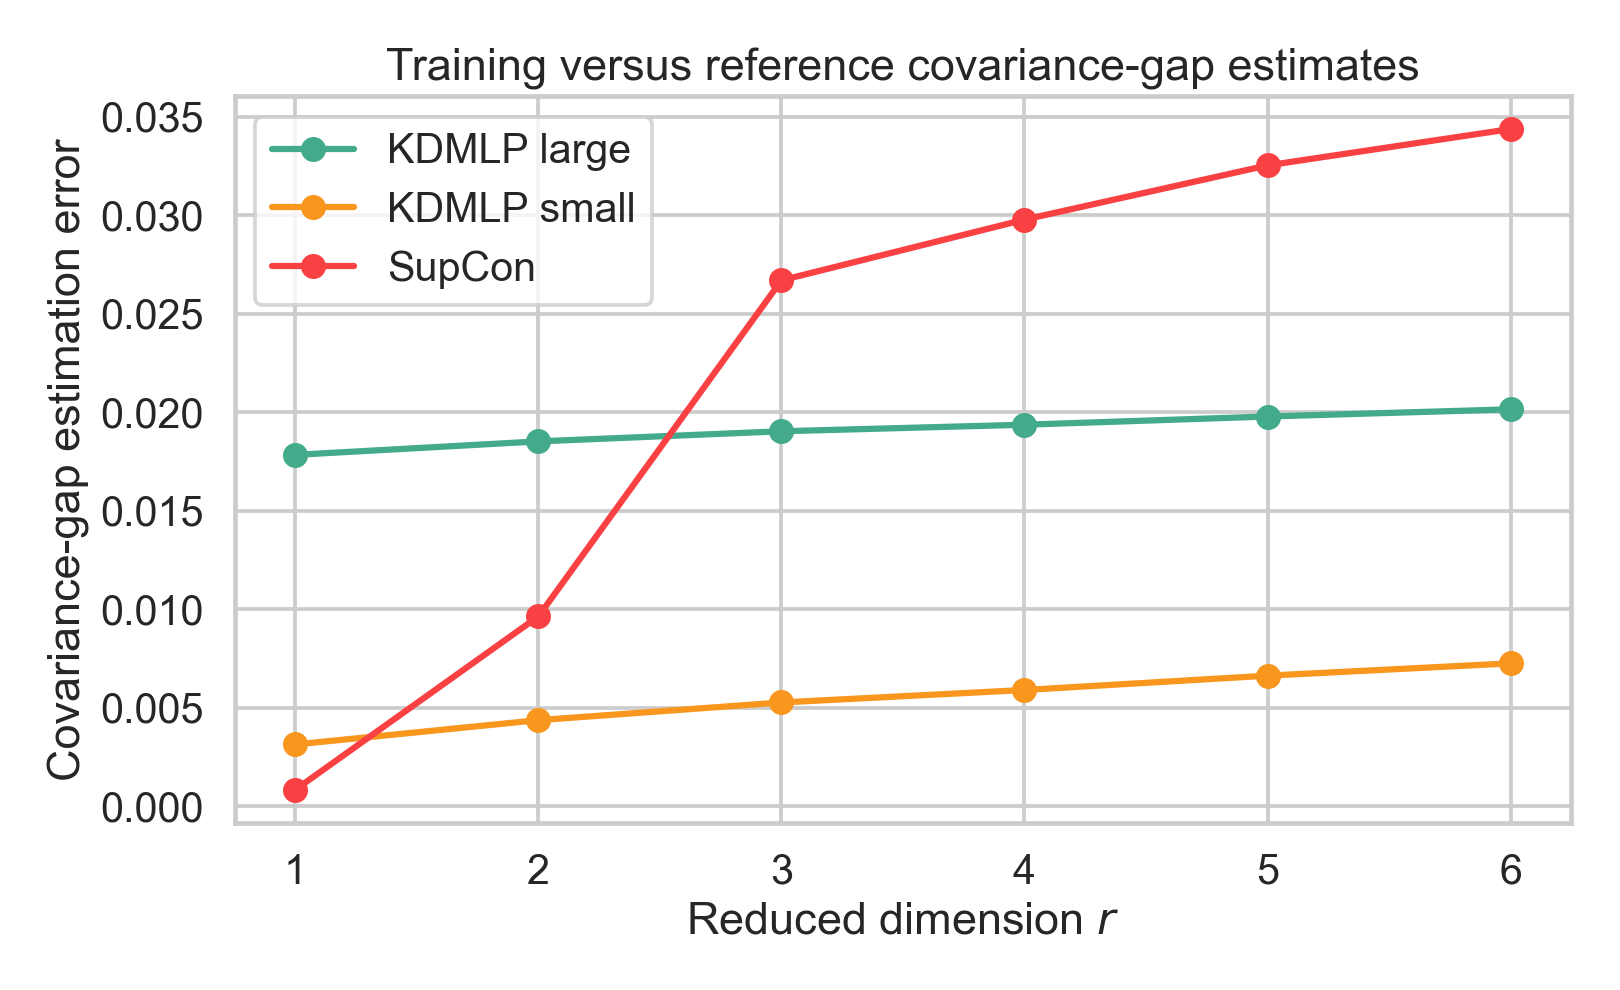
\includegraphics[width=\linewidth]{simulations/supcon_gaussian_workspace/outputs_dimmatch/same_r_covgap_error_plot.png}
 \caption{Covariance-gap estimation error.}
\end{subfigure}
\caption{Gaussian KDMLP--SupCon comparison.  Shading in the accuracy panel
denotes one standard deviation across two repetitions.}
\label{fig:gaussian-supcon}
\end{figure*}

KDMLP-large remains near $99.9\%$ accuracy from one to six dimensions, whereas
SupCon remains between $94.7\%$ and $94.9\%$.  Hence no tested SupCon dimension
matches KDMLP-large; the closest value occurs at $r=6$ and still differs by about
$0.050$.  The weaker KDMLP-small curve also shows that the advantage is not due
to dimension alone: selecting the appropriate KDMLP regime is important.  These
curves are exploratory upper envelopes because the current script chooses the
best KDMLP Stage-1 kernel at each $r$ using test accuracy; a confirmatory run
should perform this selection by nested training validation.
